\documentclass{article}
\usepackage[utf8]{inputenc}
\usepackage[T1]{fontenc}
\usepackage[english]{babel}
\usepackage[table]{xcolor} % Add this for table coloring support
\usepackage{colortbl}      % Add this for colored tables
\usepackage{hyperref}
\usepackage{bookmark} % Fixes rerunfilecheck warning for outlines
\usepackage{graphicx}
\usepackage{float}
\usepackage[hypcap=false]{caption}
\usepackage{tikz} % Added for tikzpicture environment
\usepackage{pgfplots} % Added for axis environment in tikzpicture
\graphicspath{{img/}}

\title{Exploration and Analysis of public data on Water Quality}
% Custom title page for internship report
\usepackage{fancyhdr}
\usepackage{geometry}
\usepackage{tikz}
\usepackage{setspace}

% Remove default title
\makeatletter
\renewcommand{\maketitle}{%
    \begin{titlepage}
        \thispagestyle{empty}
        \begin{tikzpicture}[remember picture,overlay]
            \node[anchor=north west, xshift=1cm, yshift=-1cm] at (current page.north west) {
                \includegraphics[height=5.5cm]{logomia.jpg} % Replace with your logo file
            };
        \end{tikzpicture}
        \vspace*{3.5cm}
        \begin{center}
            \Huge\bfseries
            Internship Report\\[1.5em]
            \LARGE
            \@title\\[2em]
            \normalsize
            \textbf{Author:} Desrosiers Jeremy\\[1em]
            \textbf{Internship Period:} 2 June 2025 -- 22 July 2025\\[1em]
            \textbf{Institution:} Laboratoire MIA - University of La Rochelle\\[1em]
            \vfill
            \large
            \@date
        \end{center}
        \vspace*{1cm}
    \end{titlepage}
}
\makeatother
\date{\today}

\begin{document}

\maketitle

\newpage
\tableofcontents
\newpage

\section{Introduction}
This internship was done in the context of the MIX Master 1st year at the University of La Rochelle.
It started on the 2nd of June 2025, and will end on the 22nd of July 2025. Hence, this report, completed the 27th of June, shows an incomplete work, that will be continued afterwards.

The goal of this internship is to analyze the water quality data in France, and to explore it in various ways, to obtain more information on water quality than the boolean 'Potable or Not Potable'. 
It's also to create and prepare tools for analyzing the data in future potential work in mind. The main focus is on the potability of water, and it's relation to the regulations in place in France and the European Union.
It covers data analysis, computer science and statistics, as well as some machine learning.

Due to the uncomplete nature of this report, it will not cover all the aspects of the internship, but will focus on the data preparation and exploration, as well as the first steps of analysis.

\section{Data Preparation}
The first step was to find the public data available on the subject, to understand and explore it, and to prepare it for analysis.
Multiple sources were provided by the intership supervisor, to start with.
\begin{itemize}
    \item \href{https://hubeau.eaufrance.fr/}{\textbf{Hubeau API:}} -- The main API for water data in France, providing access to various datasets related to water quality. \footnote{\url{https://hubeau.eaufrance.fr/}}
    \item \href{https://www.service-public.fr/particuliers/vosdroits/R11461}{\textbf{Government service:}} --  It's a governmental service that shows the latest information on water quality in France, for the selected commune. It uses the Hubeau API. \footnote{\url{https://www.service-public.fr/particuliers/vosdroits/R11461}}
\end{itemize}

None of theses sources were directly usefull, since we're looking for databases, containing the whole data, and not an API that is usefull for querying subsets of the data.
However it referenced the database used by the Hubeau API.

\newpage
\subsection{Databases}
The Hubeau API provides access to various datasets related to water quality in France, which comes from different databases.
Most of the data comes from the French public open data portal (\href{https://www.data.gouv.fr/}{data.gouv.fr}\footnote{\url{https://www.data.gouv.fr/}}), provided by the Ministry of Solidarity and Health. But other sources come from different institutions such as ADES (\href{https://ades.eaufrance.fr/}{Accès aux Données sur les Eaux Souterraines}\footnote{\url{https://ades.eaufrance.fr/}}), which is responsible for monitoring groundwater levels and quality.
In France, the water quality legally obligated to be monitored, with measurements being taken regularly all over the country.
Theses measurements takes place at different stages of the water treatment process. As shown in the following diagram:

\begin{center}
    \includegraphics[width=\textwidth]{Process_eau.png}
\end{center}
We listed the main databases related to water quality in France:
\begin{itemize}
    \item (\href{https://www.data.gouv.fr/fr/datasets/resultats-du-controle-sanitaire-de-leau-distribuee-commune-par-commune/}{\textbf{Source Water Quality}}) -- Measurements taken at the source, whether groundwater or surface water. Provided by the Ministry of Solidarity and Health.\footnote{\url{https://www.data.gouv.fr/fr/datasets/resultats-du-controle-sanitaire-de-leau-distribuee-commune-par-commune/}}
    \item (\href{https://www.data.gouv.fr/fr/datasets/resultats-du-controle-sanitaire-de-leau-du-robinet/}{\textbf{Sanitary Control of Distributed Water}}) -- Measurements taken at the distribution Units or Installations before distribution. Provided by the Ministry of Solidarity and Health.\footnote{\url{https://www.data.gouv.fr/fr/datasets/resultats-du-controle-sanitaire-de-leau-du-robinet/}}
    \item (\href{https://ades.eaufrance.fr/Recherche/Index/QualitometreAvance?g=9220e3}{\textbf{Sanitary Control of Tap Water}}) -- Measurements taken at random taps within the distribution network. Provided by ADES.\footnote{\url{https://ades.eaufrance.fr/Recherche/Index/QualitometreAvance?g=9220e3}}
\end{itemize}

\newpage
\subsection{SANDRE Referentials}
All data related to water quality in France is organized according to the SANDRE
(Service d’Admin- -istration Nationale des Données et Référentiels sur l’Eau) framework. SANDRE is a national authority responsible for establishing and maintaining standardized reference systems for all aspects of water data, including water sources, treatment facilities, distribution networks, and the parameters used to assess water quality.

The SANDRE referential ensures that every parameter relevant to water quality is assigned a unique identifier, known as \texttt{cdparametre}. This code allows for the unambiguous identification of each measured element—whether it is a physical, chemical, or biological parameter—across all datasets.

The referential is publicly accessible, and SANDRE provides an access to theses referential, as a database of an API, on it's (\href{https://www.sandre.eaufrance.fr/v2/}{website}\footnote{\url{https://www.sandre.eaufrance.fr/v2/}}. It plays an essential role in managing the afformentioned databases.

\subsection{Legislation}
We're also looking for the specific legislation that defines the water potability.
The French and European regulations diverges, on the number of parameters included, and on their limit values.

The specific Regulations can be found in the following links:
\begin{itemize}
    \item \href{https://www.legifrance.gouv.fr/loda/id/JORFTEXT000000274485/2022-11-28/}{\textbf{French Regulations on Drinking Water}}\footnote{\url{https://www.legifrance.gouv.fr/loda/id/JORFTEXT000000274485/2022-11-28/}}
    \item \href{https://eur-lex.europa.eu/FR/legal-content/summary/drinking-water-essential-quality-standards.html}{\textbf{European Regulations on Drinking Water}}\footnote{\url{https://eur-lex.europa.eu/FR/legal-content/summary/drinking-water-essential-quality-standards.html}}
\end{itemize}

Theses regulations define the maximum allowed values for microbiological parameters (the presence of dangerous organisms), aswell as chemical parameters.
The full list of values, parameters regulated, and differences are available in the annex.

\subsection{Data Selection}

For the purposes of this internship, we chose to focus our efforts on the \textbf{Sanitary Control of Distributed Water} dataset. 
This dataset is what's currently being used to determine the water potability in each communes, by the regulation authorities, which is the subject of our project.
We will of course make extensive use of the SANDRE database itself to naviguate and process the data.
On the aside, the \href{https://geo.api.gouv.fr/}{Geo.api.gouv.fr} is being used for all mapping, aswell as more data from data.gouv.fr for the communes populations notably.

\newpage
\section{Data Exploration}
A good understanding of the dataset structure, and the SANDRE framwork, is essential to perform any analysis on the data. We will describe the key elements of the dataset and framework here.
\subsection{Sanitary Control of Distributed Water dataset}
The Sanitary Control of Distributed Water dataset contains measurements from 2016 to 2025. Theses are performed at various distribution units, before distribution.
A data entry is one measurement, at one place and time, for one parameter.
Multiple measurements are done on the same sampled water, but not all parameters are measured as there are different purporses for the samples, aswell as different methods.

A consequence of that is the lack of homogeneity in the dataset. We cannot easily compare different parameters to one another, since we do not have measurements for all parameters at the same time and place.
The dataset is also not complete, as some communes do not have measurements for all parameters, and some communes do not have measurements at all, since the measurements are done at the distrubution units, often responsible for the water network of multiple communes.
Hence, in order to have data for all communes, it is needed to extrapolate the measurements on the distributed networks, also provided in the database.
But different parameters are measured at different places in the distribution network, making it hard to extrapolate accuratly the measurements to all communes concerned.
This specificity makes it difficult to extrapolate accuratly the measurements to all communes concerned. And also due to time constraint, we decided not to, to make the analysis simpler.

The dataset is ~19.7Gb in size, separated into multiple CSV files, organized by year and departement.
This size constraint was present during the whole project, as we had to process the data in chunks, and keep that separated files structure to avoid memory issues.


\subsection{Legislation}
The legislations only defines a maximum concentration allowed for some specific substances and microbiological elements. 
We first had to link theses parameters to their corresponding SANDRE code, as described afterwards.
All regulated parameters in France are present in the SANDRE referential, and are obligated to be measured, which as a direct consequence, means the measurements are present in our dataset, with a good enough sample size, both geographically and temporally.
But not all regulated parameters in Europe are, or have enough sample size.
Here's a list of all the parameters we won't be able to cover, due to insufficient sample size, or not being measured at all in the dataset.

\begin{table}[htbp]
\centering
\begin{tabular}{|l|l|}
\hline
\textbf{Not measured} & \textbf{Insufficient Sample Size} \\
\hline
Épichlorhydrine & Bisphénol A \\
Acides haloacétiques (AHA) & Chlorates \\
Pesticides & Chlorites \\
Total PFAS & Microcystine-LR \\
Hydrocarbures aromatiques polycycliques & Somme PFAS \\
 & Uranium \\
\hline
\end{tabular}
\caption{Regulated parameters not measured or with insufficient sample size in the dataset}
\end{table}

\subsection{SANDRE Parameters}
SANDRE provides an extensive list of parameters, some of which are not relevant to our analysis, and some that are not even measured in the dataset.
There's a great variety of parameters, ranging from physical parameters (e.g., temperature, pH), chemical parameters (e.g., nitrates, heavy metals), to biological parameters (e.g., presence of bacteria).
We made 2 main groups of parameters, determined in the way their measures are taken, and how they are used in the analysis.
\begin{itemize}
    \item \textbf{Continuous Parameters}: Parameters that are measured as continuous values over time (e.g., temperature).
    \item \textbf{Detected Parameters}: Parameters typically measured to detect their presence, resulting in values that are mostly zero except when detected (e.g., certain contaminants or pollutants).
\end{itemize}

Theses 2 types are important to distinguish, as they require different analysis methods.
An important focus on sample size is also nescessary, both geographically and temporally.

So, we decided on 3 filters to determine the parameters to keep:
\begin{itemize}
    \item \textbf{Temporal Sample Size}: The average number of measurements of the parameter for each commune.
    \item \textbf{Geographical Sample Size}: The number of communes where the parameter is measured.
    \item \textbf{\% non-zero values}: The percentage of non-zero measurements of the parameter. Used to determine the type of numerical data.
\end{itemize}

We processed the entire dataset to obtain theses criterias for each parameter, with thresholds on all 3 filters. At least 10 measurements per commune, for the temporal sample size, at least 12500 communes covered, for the geographical sample size, and a threshold of 15\% non-zero values, to determine the type of numerical data.

We ended up with 22 continuous parameters, and 117 detected parameters, of which, most legislated parameters are included.
The entire list of parameters is available in the annex.

The following graphs shows the distributions of the parameters in all 3 criterias.
\newpage
\subsubsection*{Continuous Parameters distribution on the 3 criterias}

\begin{center}
    \centerline{\includegraphics[width=1.0\textwidth]{average_per_commune_const.png}}
    \centerline{\includegraphics[width=1.0\textwidth]{total_communes_const.png}}
    \centerline{\includegraphics[width=1.0\textwidth]{percentage_zero_values_const.png}}
\end{center}


\newpage
\subsubsection*{Detected Parameters distribution on the 3 criterias}

\begin{center}
    \centerline{\includegraphics[width=1.0\textwidth]{average_per_commune_detect.png}}
    \centerline{\includegraphics[width=1.0\textwidth]{total_communes_detect.png}}
    \centerline{\includegraphics[width=1.0\textwidth]{percentage_zero_values_detect.png}}
\end{center}

\newpage
\section{Analysis Methods}
The entirety of the code was done in Python, using libraries such as pandas, for managing datasets, numpy, to operate on some data, and scikit-learn for analysis methods.
The analysis methods are divided into 3 main categories, each with its own focus and approach:
\begin{itemize}
    \item \textbf{Potability Analysis}: Focuses on the potability of water, as defined by the French and European regulations. It involves mapping exceedances of legal limits for each commune and parameter.
    \item \textbf{Temporal Analysis}: Centers on the temporal aspect of measurements, analyzing trends, seasonality, and correlations over time.
    \item \textbf{Correlation Analysis}: Aims to identify relationships between different parameters, particularly over time, using correlation methods suitable for time series data.
\end{itemize}

The geographical analysis wasn't a priority, and such is not present in this report. We will talk about it in the future work section.

\subsection{Potability Analysis}
We first had to see the result of current regulations, by mapping the exceedances of the legal limits for each commune, and for each parameter.
We used the geo.api.gouv.fr API to get the geographical coordinates of each communes, aswell as the geopandas python library to map it.

Due to the limited amount of data (~15 measurements over 9 years per communes), we cannot accurately determine periods of non-potability, as the measurements are not frequent enough for most parameters.
Therefore, we decided to simply count the number of exceedances of the legal limits for each commune and for each parameter.
This approach allows us to identify the communes with the highest number of exceedances, as well as the parameters that are most frequently exceeded.

\subsection{Temporal Analysis}
Temporal analysis involves the parameter, deprived of any geographical involvement. Which means that the first step is to de-regionalize the data, allowing us to only focus on the temporal aspect of the measurements.

To do that, we centered reduced the data around the mean and standard deviation of each commune individually, and then aggregated all entries into a single set.
Because we need the mean and standard deviation by commune, this implies a decent sample size by communes.
Thus we set a minimum threshold, to decide which communes to keep.

The data is also smoothed using a rolling window, to reduce noise, making any pattern clearer. To remove the outliers, we took the window of 3 times the standard deviation, centered around the mean, which means, for a centered reduced data, any value > 3.0 and < 3.0.
From this point onward, we can perform a series of timeseries analyses.

\newpage

\begin{itemize}
    \item Linear regression to identify trends over time. The scikit-learn python library provides a simple linear regression model that can be used to fit the data and identify trends.
    \item Fourier analysis from scikit-learn, to detect seasonal patterns and periodicities in the data for continuous parameters, as the detected parameters are not continuous over time. The numpy library provides a Fast Fourier transform (FFT) implementation that can be used to analyze the frequency components of the data. The peak is then detected, and a period in days is computed.
    \item Seasonal average, to compute a visual representation of seasonality for Detected parameters. Each data is aggregated by season, and the average is computed.
\end{itemize}



\subsection{Correlation Analysis}
Correlation analysis for timeseries aims to identify relationships between different parameters, 
particularly over time. Hence we used the Pearson correlation, which can detect correlations with any ammount of lag.

However, strong correlations can arise simply due to shared seasonality or trends. 
To obtain meaningful results, it is essential to detrend and deseasonalize 
the data beforehand, ensuring that observed relationships 
reflect genuine interactions rather than coincident temporal patterns.
This however wasn't done in time for this report, so only correlations for Continuous and not Seasonal parameters were done.

We also need a centered reduced and de-regionalized data, as described in the previous section, to avoid any geographical bias.

Note that making a correlation matrix requires a significant amount of memory,
since we have to process all possible pairs of parameters.
There was a significant effort toward optimizing the memory usage algorithmically. The code is present in the annex.

\newpage
\section{Results}

\subsection{Potability}
\subsubsection{French Legislation}
For the potability defined by the French legislation, we do not expect to see a lot exceedances in the measurements, since water treatement is subject to several controls resulting from theses specific measurements.
However, we still found 2 parameter with a substancial ammount of measurements exceeding the allowed Limit.

\centerline{\includegraphics[width=0.8\textwidth]{fr_1382_17.png}}

'Chlorure de Vynile' is the most exceeded parameter, with over 4\% of the measurements exceeding the legal limit of 0.5 ~$\mu$g/l. It is a known contaminant, used in the production of PVC, and that had many incidents in the past.
'Plomb' does not have a significant sample size, with only 120 measurements in the department. But the legal limit of 10 ~$\mu$g/l have been exceeded 5 times, mostly in communes distributing big cities, such as Saintes, La Rochelle and Rochefort.

So we analyzed the data per commune, in relation to it's population, on multiple parameters.
We conducted a weighted linear regression on the Concentration of 'Plomb' x Population. (weighted to compensate for the lower ammount of highly populated communes)
We however, didn't find any correlation.

\newpage
\begin{figure}[H]
    \centering
    \includegraphics[width=0.7\textwidth]{1382_population.png}
    \caption*{Concentration of Plomb vs Population}
\end{figure}

\vspace{-1em}

\noindent
On the subject of the link between the population and the concentration of certain substances, the most notable correlations we found were for 'Sulfates', 'Sodium', 'Potassium', and 'Chlorures':

\begin{figure}[H]
    \centering
    \begin{minipage}{0.48\textwidth}
        \centering
        \includegraphics[width=0.95\textwidth]{1338_population.png}
        \caption*{Sulfates}
    \end{minipage}
    \hfill
    \begin{minipage}{0.48\textwidth}
        \centering
        \includegraphics[width=0.95\textwidth]{1375_population.png}
        \caption*{Sodium}
    \end{minipage}
\end{figure}

\newpage

\begin{figure}[H]
    \centering
    \begin{minipage}{0.48\textwidth}
        \centering
        \includegraphics[width=0.95\textwidth]{1367_population.png}
        \caption*{Potassium}
    \end{minipage}
    \hfill
    \begin{minipage}{0.48\textwidth}
        \centering
        \includegraphics[width=0.95\textwidth]{1337_population.png}
        \caption*{Chlorures}
    \end{minipage}
\end{figure}

\subsubsection{European Legislation}
The european set a lower concentration for 'Plomb', of 5 ~$\mu$g/l, for which 
The Plomb is limited to 10~$\mu$g/l, but across 120 measurements in the department, with 20 measurements exceeding that limit.

When comparing the results with the European legislation, we see a small increase in the number of exceedances overall, mostly due to that parameter.
\begin{center}
\begin{minipage}{0.48\textwidth}
    \centering
    \includegraphics[width=\textwidth]{fr_17.png}
\end{minipage}\hfill
\begin{minipage}{0.48\textwidth}
    \centering
    \includegraphics[width=\textwidth]{eu_17.png}
\end{minipage}
\end{center}

\newpage

Here is the table of the number of measurements exceeding the legal limit for the previously mentionned parameters, in France, for the European regulations.

\begin{table}[H]
\centerline{\begin{tabular}{|l|l|l|l|l|}
\hline
\textbf{Parameter} & \textbf{EU/FR} & \textbf{Total Measurements} & \textbf{Over Limit Measurements} & \textbf{Percentage} \\
\hline
Plomb & EU & 142623 & 8904 & 6.24\% \\
Plomb & FR & 142623 & 2879 & 2.01\% \\
Nickel & -- & 147963 & 1906 & 1.28\% \\
Somme Pesticides & -- & 433112 & 3358 & 0.77\% \\
Chlorure de Vinyle & -- & 316466 & 14584 & 4.60\% \\
\hline
\end{tabular}}
\caption{Number and percentage of measurements exceeding the legal limit for selected parameters, in France, 2016-2025}
\end{table}

We can see a some very high percentages, especially for 'Plomb' and 'Chlorure de Vinyle'.

\subsection{Seasonality of Continuous Parameters}
One of the most interesting set of parameters are the continuous ones. The substances measured are generally always present in the water, the problematic is when their concentration is too high.
So we want to see how often the concentration of theses parameters comes close to the legal limits, and their evolution over time, to see if there's a period of the year where the concentration is higher.

For this, we widen our focus to the entire dataset, not just the communes of the Charente-Maritime department.

First of all, about the seasonality of the parameters, the most obvious one is the temperature, and all parameters that are related to it, such as the pH.
We performed a Fourier analysis of the centered-reduced and smoothed data per commune, to detect if a period of frequency equivalent to a year, is present in the data.

The following graphs shows the plotting of the centered-reduced by commune smoothed data of the Nitrates parameter. Aswell as the result of the Fourier analysis.


\centerline{\includegraphics[width=1.0\textwidth]{1340_time_series.png}}
\vspace{1em}
\centerline{\includegraphics[width=1.0\textwidth]{1340_harmonic.png}}

The yearly periodicity is clearly visible on the time series graph, with a clear peak at the begining of the year. And it is confirmed by the Fourier analysis, with a peak at 365 days, and it's harmonics at half of that, also visible.

We conducted the same analysis on all continuous parameters, and we found a significant yearly periodicity for most of them.

\newpage
We also determined the month with the highest concentration for each parameter, to see if there's a strong seasonality in the data.

\centerline{\includegraphics[width=1.0\textwidth]{1340_yearmonth.png}}

For the Nitrates parameter, the peak is in February.
We also see the evolution of the concentration over the years, with a clear increase every year, except for 2022.

This is another element of interest, that is found on several parameters, to have such a distinct year around 2020-2022, which we can assume is related to the COVID-19 pandemic, with varying lag, but this is not concrete evidence, and it's the subject for other works.


\newpage
We can now combine the results and determine the part of the year with the highest concentration for each parameter.


\begin{figure}[H]
    \centering
    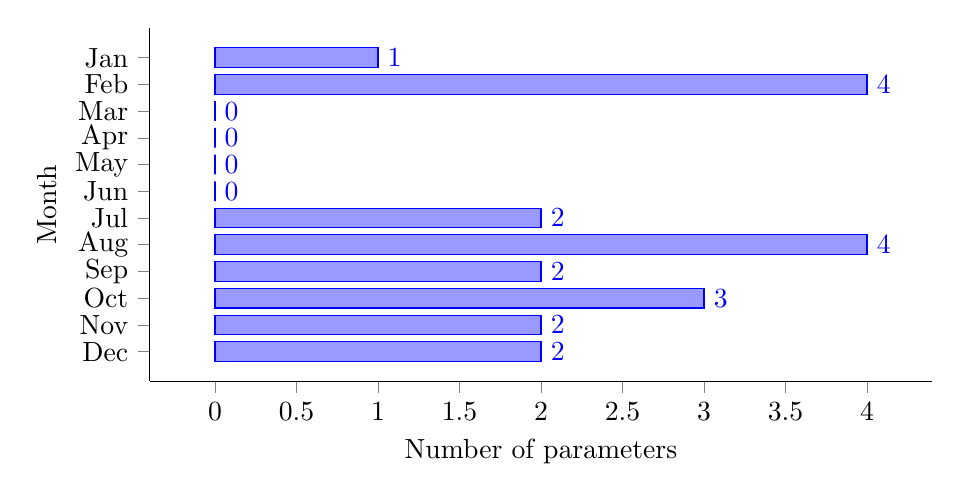
\begin{tikzpicture}
        \begin{axis}[
            xbar,
            symbolic y coords={Jan,Feb,Mar,Apr,May,Jun,Jul,Aug,Sep,Oct,Nov,Dec},
            ytick=data,
            xlabel={Number of parameters},
            ylabel={Month},
            width=0.95\textwidth,
            height=0.5\textwidth,
            bar width=0.25cm,
            nodes near coords,
            nodes near coords align={horizontal},
            axis y line*=left,
            axis x line*=bottom,
            tick align=outside,
            tick pos=left,
            y dir=reverse, % This reverses the y-axis so Jan is on top
        ]
            % Number of parameters per month
            \addplot+[xbar,fill=blue!40] coordinates {
                (1,Jan)
                (4,Feb)
                (0,Mar)
                (0,Apr)
                (0,May)
                (0,Jun)
                (2,Jul)
                (4,Aug)
                (2,Sep)
                (3,Oct)
                (2,Nov)
                (2,Dec)
            };
        \end{axis}
    \end{tikzpicture}
    \caption{Number of continuous parameters with strong seasonality, by it's peak month}
\end{figure}

\noindent
The bar height indicates the number of parameters with a strong seasonal pattern peaking in each month. For details, see the table below.

\begin{table}[H]
\centering
\begin{tabular}{|c|p{10cm}|}
\hline
\textbf{Month} & \textbf{Parameters} \\
\hline
Jan & Équilibre calcocarbonique \\
Feb & Potentiel en Hydrogène (pH), Nitrates, Chlore libre, Chlore total \\
Mar & -- \\
Apr & -- \\
May & -- \\
Jun & -- \\
Jul & Baryum, Somme des Trihalométhanes \\
Aug & Dibromochlorométhane, Température de l'Eau, Cuivre, Fluorure anion \\
Sep & Sulfates, Magnésium \\
Oct & Chlorures, Potassium, Sodium \\
Nov & Conductivité à 25°C, Dureté totale\\
Dec & Calcium, Carbone Organique \\
\hline
\end{tabular}
\caption{Parameters measured by month}
\end{table}

\section{Future Work}

So far in the internship, we have focused on the data preparation, exploration, and a first pass of analysis related to the regulations. We have identified the parameters of interest and established a framework for analyzing water quality data in relation to potability standards.

The correlation analysis was not completed in time for this report, as obtaining reliable results—especially regarding detrending and the analysis of detected parameters—requires more work. For detected parameters, the main challenge is to identify similar rare events between two parameters, potentially with a time lag, and with a non-homogeneous sample size across communes and time. So it will be the subject of future work.

Afterward, the next steps will involve the generalization of theses analysis, especially on the lacking correlation analysis across all types of parameters. And we will explore new methods, in the field of Machine Learning.

For example, the analysis of the measures of the 'Plomb' parameter, in relation to the population of the communes, could be extended to many more data, like the soil composition of the commune, the age of the water distribution network, and many other, which will make for a multi-dimensional analysis with PCA (Principal Component Analysis) and other methods.

Another important aspect was the lack of use from the RStudio python integration, which was not used at all during the internship. This will significantly simplify the analysis, as we will be able to use the R libraries for statistical geographical analysis and visualization, which are more advanced than the Python libraries.

And finally, the basis for a continuous potability index which would provide more information than the current binary potability index.

\newpage
\section{Conclusion}
This internship is a first step to create a framework for analyzing water quality data. This report comes in at the end of the first month of the internship, and is a work in progress.

The data preparation and exploration have been completed. But many more analysis is needed to satisfy the goals given. We can however give a few conclusions.

First is that the european regulations, being more strict, covers more substances, some of which are not even measured by the responsible French authorities, and thus are not present in the dataset.
Some other substances, being measured, shows a clear lack of compliance with the regulations, such as 'Plomb' and 'Chlorure de Vinyle', which are present in a significant number of communes, at about 5\% of the time.

The continuous parameters show a clear seasonality, with most peaks of concentration coming after the summer.

We also saw potential signs of the COVID-19 pandemic indirect impact on the water-quality, but this requires further investigation, as it is not conclusive yet.

\newpage

\appendix
\section{Annex}

\subsection{Parameters selected}
\subsubsection*{Continuous parameters present in legislation}
\begin{table}[H]
\centering
\begin{tabular}{|l|l|}
\hline
\textbf{Nom du paramètre} & \textbf{Code SANDRE} \\
\hline
Baryum & 1396 \\
Cuivre & 1392 \\
Fluorure anion & 7073 \\
Nitrates & 1340 \\
Somme des Trihalomethanes (4) & 2036 \\
\hline
\end{tabular}
\caption{Continuous parameters present in legislation}
\end{table}

\subsubsection*{Detected parameters present in legislation}
\begin{table}[H]
\centering
\begin{tabular}{|l|l|}
\hline
\textbf{Nom du paramètre} & \textbf{Code SANDRE} \\
\hline
Antimoine & 1376 \\
Arsenic & 1369 \\
Bore & 1362 \\
Cadmium & 1388 \\
Chrome & 1389 \\
Indice Cyanures totaux & 1390 \\
Plomb & 1382 \\
Manganèse & 1394 \\
Mercure & 1387 \\
Nickel & 1386 \\
Nitrites & 1339 \\
Sélénium & 1385 \\
Acrylamide & 1457 \\
Benzène & 1114 \\
Benzo(a)pyrène & 1115 \\
Bromates & 1751 \\
Dichloroéthane-1,2 & 1161 \\
Somme des pesticides totaux & 6276 \\
Somme du tetrachloroéthylène et du trichloroéthylène & 2963 \\
Chlorure de vinyle & 1753 \\
\hline
\end{tabular}
\caption{Detected parameters present in legislation}
\end{table}

\subsubsection*{Continuous Parameters outside of legislation}
\begin{table}[H]
\centering
\begin{tabular}{|l|l|}
\hline
\textbf{Nom du paramètre} & \textbf{Code} \\
\hline
pH d'equilibre & 6488 \\
Carbone Organique & 1841 \\
Calcium & 1374 \\
Conductivité à 25°C & 1303 \\
Titre alcalimétrique complet (T.A.C.) & 1347 \\
Hydrogénocarbonates & 1327 \\
Température de mesure du pH & 6484 \\
Equilibre calcocarbonique de l’eau destinée à la consommation humaine & 5907 \\
Potentiel en Hydrogène (pH) & 1302 \\
Potassium & 1367 \\
Sulfates & 1338 \\
Nitrates/50 + Nitrites/3 & 6374 \\
Magnésium & 1372 \\
Chlore total & 1399 \\
Chlorures & 1337 \\
Dibromochloromethane & 1158 \\
Chlore libre & 1398 \\
Température de l'Eau & 1301 \\
Dureté totale & 1345 \\
Sodium & 1375 \\
\hline
\end{tabular}
\caption{Continuous Parameters outside of legislation}
\end{table}

\subsubsection{Detected Parameters outside of legislation}
\begin{table}[H]
\centering
\centerline{
    \begin{tabular}{|l|l||l|l|}
    \hline
    \textbf{Parameter Name} & \textbf{Code} & \textbf{Parameter Name} & \textbf{Code} \\
    \hline
    Chloroforme & 1135 & Carbendazime & 1129 \\
    Nicosulfuron & 1882 & 2-hydroxy atrazine & 1832 \\
    Fluroxypyr-meptyl & 2547 & Procymidone & 1664 \\
    Ammonium & 1335 & 3,4-dichlorophenyluree & 1930 \\
    Imazamox & 2986 & Aspect de l'eau potable & 6489 \\
    Fenbuconazole & 1906 & Terbuméton & 1266 \\
    Triallate & 1281 & Chlortoluron & 1136 \\
    Flonicamid & 6393 & Triclopyr & 1288 \\
    Dichloromonobromométhane & 1167 & Dicamba & 1480 \\
    Heptachlore & 1197 & Terbuthylazine & 1268 \\
    Atrazine déséthyl & 1108 & Metconazole & 1879 \\
    Imidaclopride & 1877 & Glyphosate & 1506 \\
    Titre alcalimétrique (T.A.) & 1346 & Perméthrine & 1523 \\
    Benzo(g,h,i)pérylène & 1118 & Trinexapac-ethyl & 2096 \\
    Dinoterbe & 1176 & Flurtamone & 2008 \\
    Pyriméthanil & 1432 & Chlorpyriphos-éthyl & 1083 \\
    Malathion & 1210 & Chlorothalonil-R471811 & 8865 \\
    Métobromuron & 1515 & Imazaméthabenz-méthyl & 1911 \\
    Alachlore & 1101 & Clopyralide & 1810 \\
    DDT 24' & 1147 & Hexaconazole & 1405 \\
    Somme Heptachlore époxyde cis/trans & 1198 & Fer & 1393 \\
    Prosulfuron & 2534 & Isoxaben & 1672 \\
    Fludioxonil & 2022 & Oxyfluorfène & 1952 \\
    Pyraclostrobine & 2576 & Linuron & 1209 \\
    Prosulfocarbe & 1092 & Epoxiconazole & 1744 \\
    Piperonyl butoxyde & 1709 & Dichlorvos & 1170 \\
    2,4,5-T & 1264 & Anthraquinone & 2013 \\
    Hexachlorobenzène & 1199 & Dichlorprop & 1169 \\
    Iprodione & 1206 & Prométryne & 1254 \\
    DDE 44' & 1146 & Somme des Hexachlorocyclohexanes & 5537 \\
    Cyprodinil & 1359 & Spores micro-orga anaérobies sulfito-réduc & 1042 \\
    Bromacil & 1686 & Isoxaflutole & 1945 \\
    Desmétryne & 1155 & Quinmerac & 2087 \\
    Triadiméfone & 1544 & Couleur mesurée & 1309 \\
    Aldrine & 1103 & Bromoxynil & 1125 \\
    Deltaméthrine & 1149 & Bromuconazole & 1860 \\
    Diméthomorphe & 1403 & Trichloroéthylène & 1286 \\
    Foramsulfuron & 2806 & Boscalid & 5526 \\
    Flazasulfuron & 1939 & Florasulam & 2810 \\
    Ethofumésate & 1184 & fluxapyroxade & 7342 \\
    Tébuconazole & 1694 & Terbuthylazine hydroxy & 1954 \\
    Glufosinate & 1526 & Carbétamide & 1333 \\
    Propyzamide & 1414 & Endosulfan bêta & 1179 \\
    Diuron & 1177 & Odeur de l’eau & 5901 \\
    Benoxacor & 2074 & Prochloraz & 1253 \\
    Carbofuran & 1130 & Monuron & 1228 \\
    Méthabenzthiazuron & 1216 & Lambda-cyhalothrine & 1094 \\
    mepiquat & 1969 & Diméfuron & 1870 \\
    Atrazine 2-hydroxy-desethyl & 3159 & Terbuthylazine desethyl-2-hydroxy & 7150 \\
    Spiroxamine & 2664 & Metsulfuron méthyle & 1797 \\
    \hline
    \end{tabular}
}
\caption{Detected parameters outside of legislation. Part3}
\end{table}

\begin{table}[H]
\raggedright % Align table to the left
\setlength{\tabcolsep}{6pt} % Reduce column separation
\centerline{
    \begin{tabular}{|l|l||l|l|}
    \hline
    \textbf{Parameter Name} & \textbf{Code} & \textbf{Parameter Name} & \textbf{Code} \\
    \hline
    HAP somme(4) & 2033 & Diméthachlore & 2546 \\
    Endosulfan & 1743 & Acetochlor ESA & 6856 \\
    Propiconazole & 1257 & Pentachlorophénol & 1235 \\
    Diazinon & 1157 & Micro-organismes revivifiables à 36°C & 5441 \\
    Cyperméthrine & 1140 & Acétochlore & 1903 \\
    Métazachlore & 1670 & Chloridazone & 1133 \\
    Métribuzine & 1225 & Lénacile & 1406 \\
    Acetamiprid & 5579 & Desméthylisoproturon & 2738 \\
    Fluroxypyr & 1765 & Flusilazole & 1194 \\
    Hexazinone & 1673 & Endosulfan sulfate & 1742 \\
    Dichlobenil & 1679 & Monolinuron & 1227 \\
    DDD 24' & 1143 & KRESOXIM-METHYL & 1950 \\
    Oryzalin & 1668 & Dieldrine & 1173 \\
    2,6-Dichlorobenzamide & 2011 & Endrine & 1181 \\
    Dinitrocresol & 1490 & Cyanazine & 1137 \\
    Terbumeton désethyl & 2051 & Mesosulfuron methyle & 2578 \\
    Terbuthylazine désethyl & 2045 & AZOXYSTROBINE & 1951 \\
    Benzo(k)fluoranthène & 1117 & Aclonifène & 1688 \\
    Clethodim & 2978 & Fenoxycarbe & 1967 \\
    Terbutryne & 1269 & Secbuméton & 1262 \\
    Myclobutanil & 1881 & Simazine & 1263 \\
    Chlorpyriphos-méthyl & 1540 & Metolachlor ESA & 6854 \\
    Atrazine & 1107 & Chlorothalonil & 1473 \\
    Amidosulfuron & 2012 & Alachlor ESA & 6800 \\
    Trifluraline & 1289 & Heptachlore époxyde endo trans & 1749 \\
    Micro-organismes revivifiables à 22°C & 5440 & Métazachlore ESA & 6895 \\
    Chlorprophame & 1474 & Thiacloprid & 5671 \\
    Ioxynil & 1205 & Tritium (3H) & 2098 \\
    Atrazine déisopropyl-2-hydroxy & 3160 & Flufénacet ESA & 6864 \\
    Sulcotrione & 1662 & DDD 44' & 1144 \\
    Dicofol & 1172 & Heptachlore époxyde exo cis & 1748 \\
    2,4-D & 1141 & Dinosèbe & 1491 \\
    Bromoforme & 1122 & Hexachlorocyclohexane delta & 1202 \\
    Enterocoques & 6455 & DDE 24' & 1145 \\
    Sulfosulfuron & 2085 & Clomazone & 2017 \\
    Sébuthylazine & 1923 & Activité bêta globale résiduelle & 2955 \\
    Fénuron & 1500 & Cycloxydime & 2729 \\
    Atrazine déisopropyl & 1109 & Iodosulfuron-methyl-sodium & 6483 \\
    Métolachlore total & 1221 & Diméthénamide & 1678 \\
    Cymoxanil & 1139 & Hexachlorobutadiène & 1652 \\
    Fluoranthène & 1191 & Benzo(b)fluoranthène & 1116 \\
    Activité alpha globale & 1034 & AMPA & 1907 \\
    Tétrachloroéthylène & 1272 & Diquat & 1699 \\
    Pyroxsulam & 7340 & Hexachlorocyclohexane alpha & 1200 \\
    Tribenuron-Methyle & 2064 & Carbaryl & 1463 \\
    Amétryne & 1104 & Oxadiazon & 1667 \\
    Metolachlor OXA & 6853 & Thiafluamide & 1940 \\
        \hline
    \end{tabular}
}
\caption{Detected parameters outside of legislation. Part2}
\end{table}

\begin{table}[H]
\raggedright % Align table to the left
\setlength{\tabcolsep}{6pt} % Reduce column separation
\centerline{
    \begin{tabular}{|l|l||l|l|}
    \hline
    \textbf{Parameter Name} & \textbf{Code} & \textbf{Parameter Name} & \textbf{Code} \\
    \hline
    Mécoprop & 1214 & Saveur de l’eau & 5902 \\
    Métalaxyl & 1706 & Simazine-hydroxy & 1831 \\
    Aluminium & 1370 & Epichlorohydrine & 1494 \\
    Métaldéhyde & 1796 & Trifloxystrobine & 2678 \\
    Atrazine déisopropyl déséthyl & 1830 & Thifensulfuron méthyl & 1913 \\
    Fenpropimorphe & 1189 & Tetraconazole & 1660 \\
    Bentazone & 1113 & Fipronil & 2009 \\
    Indéno(1,2,3-cd)pyrène & 1204 & Activité bêta globale & 1035 \\
    Endosulfan alpha & 1178 & Thiabendazole & 1713 \\
    Chlormequat & 5554 & Ethidimuron & 1763 \\
    Aminotriazole & 1105 & Diflufenicanil & 1814 \\
    Cyproconazole & 1680 & asulame & 1965 \\
    Pirimicarbe & 1528 & Bifénox & 1119 \\
    Dose Totale Indicative (DTI) & 2059 & Clothianidine & 6389 \\
    Propazine & 1256 & TEFLUTHRINE & 1953 \\
    Pendiméthaline & 1234 & Escherichia coli (E. coli) & 1449 \\
    Oxadixyl & 1666 & Hexachlorocyclohexane bêta & 1201 \\
    Norflurazone & 1669 & Couleur de l’eau & 5900 \\
    Difénoconazole & 1905 & Imazaméthabenz & 1695 \\
    Métoxuron & 1222 & Alachlor OXA & 6855 \\
    Desmethylnorflurazon & 2737 & Métamitrone & 1215 \\
    Mésotrione & 2076 & Flurochloridone & 1675 \\
    DDT 44' & 1148 & Flutriafol & 1503 \\
    Quinoxyfen & 2028 & Coliformes & 1447 \\
    Propamocarb & 6398 & Turbidité Formazine Néphélométrique & 1295 \\
    Métazachlore OXA & 6894 & Thiamethoxam & 6390 \\
    Diméthoate & 1175 & 1-(3,4-dichlorophenyl)-3-methyl-uree & 1929 \\
    Chlorfenvinphos & 1464 & Fenpropidine & 1700 \\
    2,4-MCPA & 1212 & Isoproturon & 1208 \\
    Hexachlorocyclohexane gamma & 1203 & Napropamide & 1519 \\
    Carbonates & 1328 & Tébutame & 1661 \\
    \hline
\end{tabular}
}
\caption{Detected parameters outside of legislation. Part3}
\end{table}

\subsection{Summary Table: French vs European Criterias for water quality}
\begin{table}[H]
\centering
\begin{tabular}{|l|l|l|l|}
\hline
\textbf{Code} & \textbf{Substance} & \textbf{French Limit} & \textbf{European Limit} \\
\hline
1376 & Antimoine & 5,0 µg/l & 10 µg/l \\
1369 & Arsenic total & 10 µg/l & 10 µg/l \\
1396 & Baryum & 1,0 mg/l & -- \\
1362 & Bore & 1,0 mg/l & 1,5 mg/l \\
1388 & Cadmium & 5,0 µg/l & 5,0 µg/l \\
1389 & Chrome & 50 µg/l & 25 µg/l \\
1392 & Cuivre & 2,0 mg/l & 2,0 mg/l \\
1390 & Cyanures & 50 µg/l & 50 µg/l \\
7073 & Fluorures & 1,5 mg/l & 1,5 mg/l \\
1382 & Plomb & 10 µg/l & 5 µg/l \\
1394 & Manganèse & 500 µg/l & -- \\
1387 & Mercure & 1,0 µg/l & 1,0 µg/l \\
1386 & Nickel & 20 µg/l & 20 µg/l \\
1340 & Nitrates & 50 mg/l & 50 mg/l \\
1339 & Nitrites & 0,1 mg/l & 0,50 mg/l \\
1385 & Sélénium & 10 µg/l & 20 µg/l \\
1457 & Acrylamide & 0,10 µg/l & 0,10 µg/l \\
1114 & Benzène & 1,0 µg/l & 1,0 µg/l \\
1115 & Benzo(a)pyrène & 0,010 µg/l & 0,010 µg/l \\
2766 & Bisphénol A & -- & 2,5 µg/l \\
1751 & Bromates & 10,0 µg/l & 10,0 µg/l \\
1752 & Chlorates & -- & 0,25 mg/l \\
1735 & Chlorites & -- & 0,25 mg/l \\
1161 & 1,2-dichloroéthane & 3,0 µg/l & 3,0 µg/l \\
X & Épichlorhydrine & 0,10 µg/l & 0,10 µg/l \\
X & Acides haloacétiques (AHA) & -- & 60 µg/l \\
2058 & Microcystine-LR & -- & 1,0 µg/l \\
X & Pesticides & 0,10 µg/l & 0,10 µg/l \\
6276 & Total pesticides & 0,50 µg/l & 0,50 µg/l \\
X & Total PFAS & -- & 0,50 µg/l \\
8847 & Somme PFAS & -- & 0,10 µg/l \\
X & Hydrocarbures aromatiques polycycliques & -- & 0,10 µg/l \\
2963 & Tétrachloroéthylène et trichloroéthylène & 10,0 µg/l & 10,0 µg/l \\
2036 & Total trihalométhanes & 100,0 µg/l & 100,0 µg/l \\
1361 & Uranium & -- & 30,0 µg/l \\
1753 & Chlorure de vinyle & 0,5 µg/l & 0,50 µg/l \\
\hline
\end{tabular}
\caption{Summary Table: French vs European Criteria for Drinking Water}
\end{table}
\end{document}